\documentclass[11pt]{article}

\usepackage{fullpage}
\usepackage{amsfonts}
\usepackage{graphicx}

\def\eq1{y=\frac{x}{3*x^2+x+1}}
\def\labelaxes{Remember to include a scale and label to your axes.}

\begin{document}

\begin{center}
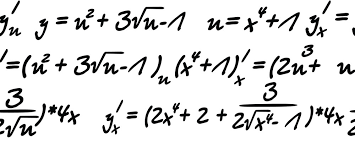
\includegraphics[scale=0.5,angle=45]{algebra.png}

Remember images must be saved as .png .jpg .pdf .gif files.
\end{center}



The set of natural numbers is denoted by $\mathbb{N}$.

The set of integers is denoted by $\mathbb{Z}$.

The set of real numbers is denoted by $\mathbb{R}$.

Graph $\eq1$. \labelaxes

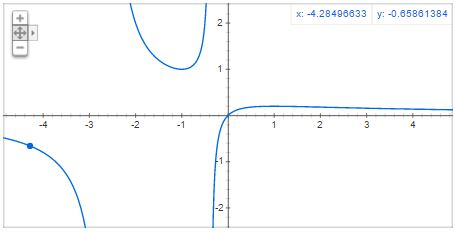
\includegraphics[width = 5in]{plot.jpg}

Identify the asymptotic for the graph of $\eq1$. 

\end{document}